\chapter{Theoretical Background}\label{chapter:background}
In this chapter, I present the definitions, concepts, and frameworks that are helpful to
understand the later parts of this thesis. After providing a brief definitional introduction of general concepts related to XR, collaboration and industry, I explore how these fields converge in the context of AR-based collaboration in industrial tasks.
I structure this work to reflect its multidisciplinary nature, which spans XR technologies, collaborative systems, and industrial applications. Finally, I provide some background on the study design, questionnaires and evaluation metrics in later chapters.

\section{Extended Reality (XR)}
\label{sec:xr}
\textit{Extended reality} (XR) is an umbrella term that describes the spectrum of immersive technologies that blend physical and digital stimuli to varying degrees. Milgram and Kishino's Reality-Virtuality (RV) continuum \cite{milgram1995augmented} (see Figure \ref{fig:rv-continuum}) positions any XR experience along an axis from the purely physical to the purely digital, while more recent syntheses emphasise multisensory integration, ubiquitous networking and edge computing as additional determinants of XR fidelity \cite{doerner2022xrTextbook}. Within this spectrum, virtual reality (VR), augmented reality (AR), and mixed reality (MR) represent key categories, each defined by how they engage users with virtual and real elements \cite{doerner2022xrTextbook}. This complements the taxonomy proposed by \cite{milgram1995augmented}, which I will briefly define in the following.

\begin{figure}[t!]
    \centering
    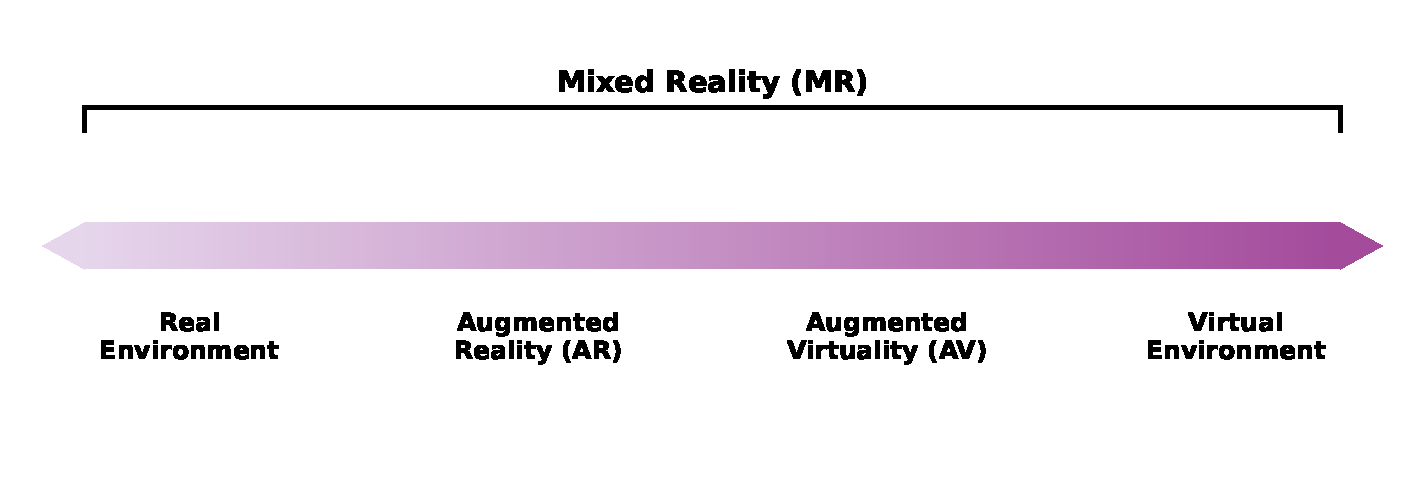
\includegraphics[width=0.8\textwidth]{assets/02/xr-cont.pdf}
    \caption{Milgram and Kishino's Reality-Virtuality (RV) continuum (Source: Based on \cite{milgram1995augmented}).}
    \label{fig:rv-continuum}
\end{figure}



\subsection{Virtual Reality (VR)}
\textit{Virtual reality} (VR) fully immerses its users in a computer-generated environment, replacing all sensory inputs from the physical world. Through devices such as HMDs, users interact with 3D virtual spaces designed for applications ranging from gaming to training simulations. The immersive nature of VR creates a controlled environment ideal for scenarios that benefit from complete isolation from real-world distractions \cite{doerner2022xrTextbook}

\subsection{Augmented Reality (AR)}
\textit{Augmented reality} (AR) overlays virtual objects onto the real world, blending the digital with the physical. Using devices like smartphones or AR-enabled HMDs, AR allows users to interact with virtual elements while being aware of their physical surroundings. This makes AR particularly valuable in applications such as real-time guidance, education, and collaborative tasks \cite{doerner2022xrTextbook}.

\subsection{Mixed Reality (MR)}
\textit{Mixed reality} (MR) combines elements of VR and AR, creating environments where virtual and real objects coexist and interact seamlessly. MR systems rely on advanced spatial tracking and computing to anchor virtual elements within the physical space, enabling applications such as hybrid collaboration and immersive design \cite{doerner2022xrTextbook}.
\vspace{4mm}

In the remainder of this thesis, I will use the term ``AR'' to broadly refer to XR systems that contain AR and MR components and are facilitated with head-mounted displays (HMDs).


\section{Industrial Assembly Processes}\label{sec:assembly}
Manual assembly remains indispensable wherever product variability,
low-volume production, or delicate operations render full automation
uneconomic. As it is often the final stage of a longer production process, errors in assembly are costly and can lead to rework or even scrap. This means that, despite decades of research on mechanisation, even today, the majority of final assembly operations in European factories are still performed by humans
\cite{fast2016evaluating}
\cite{claeys2015framework}.
Understanding assembly therefore requires both
an organisational typology of assembly systems and a task-level view
of the operator activities that comprise an assembly cycle.

\subsection{Assembly-system typology}\label{subsec:typologies}
Following \cite{hu2011assemblySystemVariety}, \cite{pilati2021multi} and \cite{greene1984review}, I distinguish four generic
system configurations:
\begin{description}
  \item[Synchronous~(paced) lines] every product follows an identical, clocked
        sequence, advancing in lock-step between stations.  This layout suits
        high-volume, low-variety production, but affords little flexibility.
  \item[Asynchronous lines] parts can follow alternative paths and dwell times
        vary by workstation, improving robustness to disturbances and
        supporting mixed-model production.
  \item[Concurrent or multi-manned lines] multiple operators work
        simultaneously on the same product within a workstation, enabling
        parallel execution of precedence-independent tasks and shortening
        cycle times—common in large-scale assemblies such as vehicle bodies
        \cite{michels2020multiManned}.
  \item[Cellular systems] machines and workers are clustered into
        cells that each complete a family of similar products in
        one-piece flow, yielding flexibility and reduced material transport
        \cite{liker2004toyota}.
\end{description}

\subsection{Phases of manual assembly}\label{subsec:phases}
Irrespective of the macro-layout, individual operators typically alternate
between two cognitive-motor phases\cite{boothroyd2010product}:
\begin{enumerate}
  \item \textbf{Commissioning (kitting or picking)}—locating and
        retrieving the required components or tools.  Efficient kitting has
        been shown to reduce search time and error rates in high-variety
        assembly\cite{wilhelm1992kitting}.
  \item \textbf{Joining (fitting or fastening)}—physically integrating
        parts according to the assembly plan.  Errors in this phase account
        for the majority of rework costs\cite{stork2010cognitionInAssembly}.
\end{enumerate}
I therefore consider how AR interventions may target either phase. For example, visual pick-by-light
systems could support commissioning, whereas step-wise holographic instructions
could support joining \cite{hanson2017augmented}\cite{dalle2021augmented}.



\section{Collaboration, Cooperation, and Teamwork}\label{sec:collab}
The literature differentiates cooperation—a division of labour among
individuals pursuing compatible goals—from collaboration, where
participants engage mutually in a coordinated effort to construct
shared understanding and jointly solve a problem~\cite{roschelle1995construction}.  Johnson and Johnson's social interdependence theory further
emphasises positive goal interdependence, individual accountability, and
promotive interaction as hallmarks of effective cooperation\cite{johnson1989cooperation}.  In industrial practice, cooperative work is
exemplified by parallel sub-assembly, whereas collaboration arises when
operators synchronously negotiate and adapt their actions on a shared work
object. This latter will be the focus of this thesis.

Spatial (co-located vs. remote), temporal (synchronous vs. asynchronous),
informational (symmetric vs. asymmetric), and technological (optical vs.
video see-through, projection) dimensions provide an organising framework
for analysing collaborative settings\cite{feng2023comprehensive,samini2021review,roschelle1995construction}.


\section{AR-Supported Industrial Tasks}\label{sec:ar_industrial}
Technological advancements have played a large role in shaping manual assembly processes. Computer-aided planning and monitoring systems, for example, have improved process control, increased efficiency, and facilitated data collection~\cite{kärcher2018sensorDriven, Yong-liang2009Computer}. More recently, cognitive support systems such as augmented reality (AR) have been increasingly applied to further reduce operator workload, enhance accuracy, and optimise task sequences~\cite{stork2010cognitionInAssembly}.
AR technologies have found applications throughout the industrial lifecycle, including design reviews, maintenance, training, inspection, and especially manual assembly~\cite{deSouza2020surveyIndustrialAR, cim2024arAssemblyTrainingRev}. In these contexts, AR provides cognitive guidance through spatially registered overlays, which can reduce mental workload and decrease task-switching latency~\cite{stork2010cognitionInAssembly, tang2003comparative}. 
Despite these benefits, the effectiveness of AR support is limited by human perceptual and ergonomic constraints. Furthermore, integrating AR systems into heterogeneous production environments remains a notable research challenge~\cite{mekni2014augmented, al2025investigating}.


\section{AR-Based Collaboration}\label{sec:ar_collab}
Building on the dimensions in Section~\ref{sec:collab}, AR-based collaboration can be characterised along multiple dimensions that influence both the design and effectiveness of collaborative systems. These dimensions provide a comprehensive framework for understanding how AR technologies can support different collaborative configurations in industrial contexts.

\subsection{Spatial and Temporal Dimensions}
AR collaboration can take many forms, depending on the physical location of participants and the mode of interaction \cite{feng2023comprehensive}. The spatial dimension distinguishes between \textit{remote} and \textit{co-located} collaboration:

\begin{itemize}
    \item \textit{Remote collaboration} occurs when collaborators are in different physical locations, with AR used to bridge the gap through shared virtual spaces. For example, a remote team can work together on a virtual prototype or troubleshoot equipment using AR overlays, enabling expert guidance without physical presence.
    \item \textit{Co-located collaboration} involves participants physically present in the same location, using AR to enhance their shared environment and exchange information. This might include overlaying step-by-step instructions for assembling machinery or visualising complex data in real-time.
\end{itemize}

The temporal dimension further distinguishes between \textit{asynchronous} and \textit{synchronous} interaction modes \cite{feng2023comprehensive}:

\begin{itemize}
    \item \textit{Asynchronous collaboration} allows participants to interact with the AR system at different times. This is commonly used to leave instructions, notes, or annotations for others to review later, enabling a flexible workflow that accommodates different schedules and time zones.
    \item \textit{Synchronous collaboration} occurs in real-time, with all participants interacting with the AR system and each other simultaneously. This is especially valuable in scenarios that require immediate feedback or cooperative problem-solving.
\end{itemize}

\subsection{Technological Dimensions}
The choice of device facilitating the AR interface has a large impact on the collaboration experience \cite{samini2021review}. Three primary technological approaches can be distinguished\cite{azuma1997survey}\cite{bimber2005spatial}:

\begin{itemize}
    \item \textit{Video see-through (VST)} devices use cameras to capture the real world, combining this video feed with virtual overlays on display. This includes hand-held devices (HHD) like smartphones and tablets, as well as various HMDs equipped with cameras.
    \item \textit{Optical see-through (OST)} devices employ semi-transparent displays that allow users to see the real world directly while adding computer-generated overlays. This approach provides more natural depth perception but may suffer from brightness and contrast limitations.
    \item \textit{Projection-based} systems display augmentations directly onto real-world surfaces without requiring head-worn or handheld displays. These systems can support multiple users simultaneously but are limited by environmental lighting conditions and surface characteristics.
\end{itemize}

\subsection{Information Symmetry and Collaboration Modes}
The distribution of information among collaborators represents another critical dimension. Access to information can be either \textit{symmetric} or \textit{asymmetric} \cite{feng2023comprehensive}:

\begin{itemize}
    \item \textit{Symmetric information sharing} gives all participants access to the same information, creating a level playing field for collaboration and supporting equality in decision-making processes.
    \item \textit{Asymmetric information sharing} provides some collaborators with more detailed or specific data, such as when an expert has access to diagnostic overlays while a trainee views basic instructions. This approach supports hierarchical collaboration and guided learning scenarios.
\end{itemize}

Building on these dimensions, human-human collaboration in AR assembly can occur in various configurations (see Figure~\ref{fig:ar-collab-modes}):

\begin{itemize}
  \item \textbf{Remote AR-AR collaboration}: Distributed teams manipulate a shared holographic workspace, enabling applications such as tele-maintenance and distributed design reviews.
  \item \textbf{Co-located AR-AR collaboration}: All collaborators perceive identical augmentations in the same physical space, promising for synchronised assembly or quality control where spatial coordination is crucial.
  \item \textbf{Hybrid AR-non-AR collaboration}: One operator wears an HMD while peers use conventional tools, requiring careful information symmetry design to ensure effective communication and coordination \cite{aschenbrenner2018collaborative}.
\end{itemize}

\begin{figure}[t!]
    \centering
    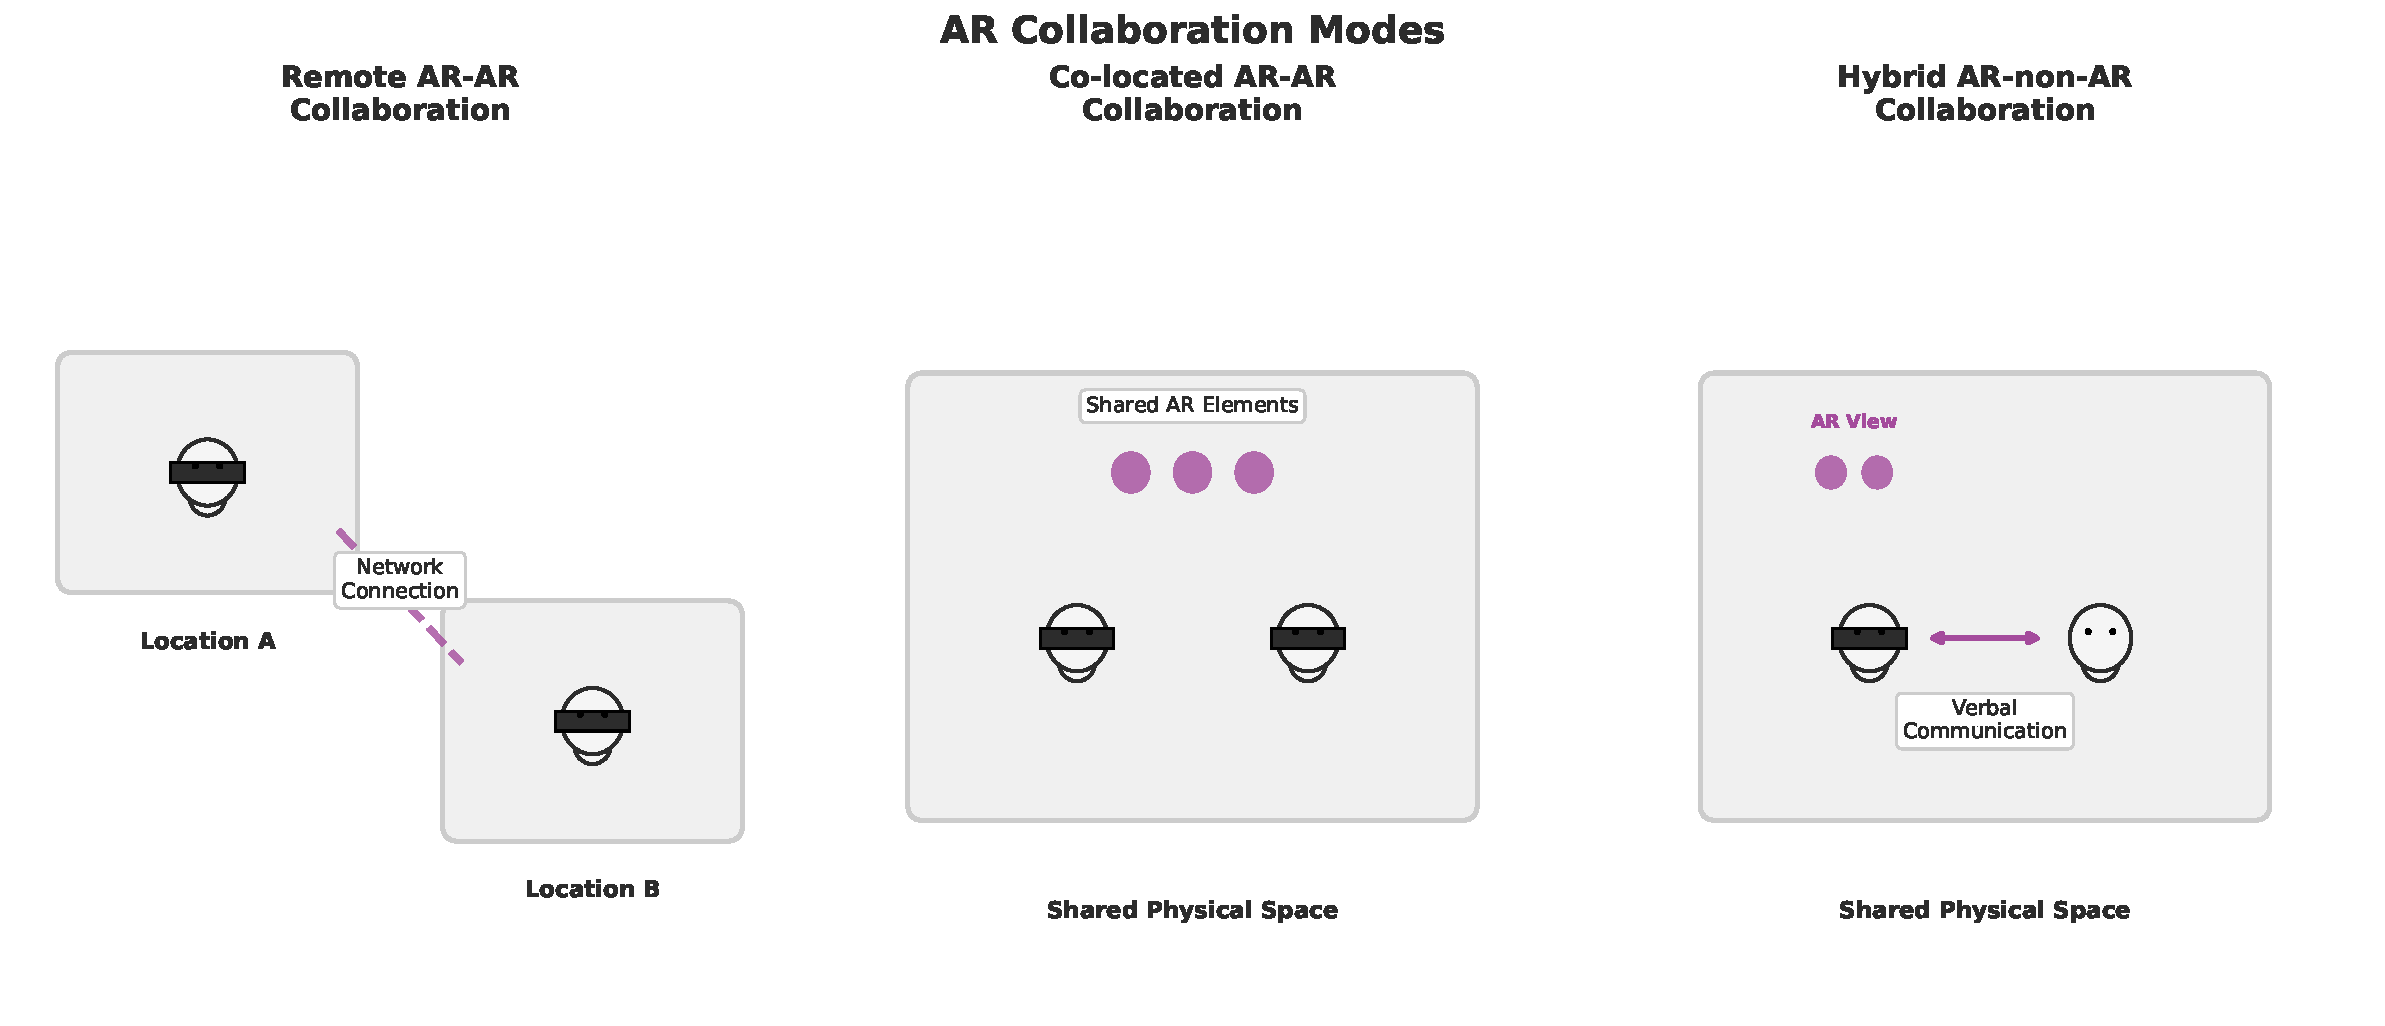
\includegraphics[width=0.9\textwidth]{assets/02/ar-collaboration-modes.pdf}
    \caption{AR collaboration modes illustrating the three primary configurations for human-human collaboration in AR environments.}
    \label{fig:ar-collab-modes}
\end{figure}

Prior research has acknowledged the usefulness of collaborative AR technologies in an assembly context \cite{wang2016arAssemblyLitRev}. Nevertheless, in an industrial context, most prior work targets human-robot interaction, with AR visualising robot intent or remotely tele-operating manipulators \cite{schmidt2022augmentedReality}. Purely human-human AR collaboration remains underexplored—particularly concerning how shared augmentations influence division of labour, joint attention, and situation awareness in manual assembly.


